\documentclass[11pt]{article}

\usepackage[T1]{fontenc}
\usepackage[utf8]{inputenc}
\usepackage{lmodern}
\usepackage{microtype}
\usepackage[margin=1in]{geometry}
\usepackage{booktabs}
\usepackage{array}
\usepackage{amsmath}
\usepackage{xcolor}
\usepackage{tikz}
\usepackage{pgfplots}
\usepackage{listings}
\usepackage{enumitem}
\usepackage{fancyhdr}
\usepackage[colorlinks=true,linkcolor=blue!60!black,urlcolor=blue!60!black]{hyperref}

\pgfplotsset{compat=1.17}
\definecolor{codebg}{RGB}{246,248,250}
\definecolor{codekeyword}{RGB}{175,0,219}
\definecolor{codestring}{RGB}{032,102,058}
\definecolor{codecomment}{RGB}{098,098,098}

\lstdefinestyle{python}{
  language=Python,
  basicstyle=\ttfamily\footnotesize,
  backgroundcolor=\color{codebg},
  keywordstyle=\color{codekeyword}\bfseries,
  stringstyle=\color{codestring},
  commentstyle=\color{codecomment}\itshape,
  showstringspaces=false,
  breaklines=true,
  columns=fullflexible,
  frame=single,
  rulecolor=\color{gray!40},
  aboveskip=0.7em,
  belowskip=0.7em,
}

\newcommand{\code}[1]{\texttt{#1}}
\newcommand{\run}{\texttt{Run(ctx, a)}}

\title{\bfseries Python Code Mode Harness Replay\\
\large The 2026-11-19 arm and scenario matrix on the current build}
\author{enuma-elis harness corpus}
\date{2026-11-19}

\pagestyle{fancy}
\fancyhf{}
\fancyhead[L]{Python Code Mode Harness Replay}
\fancyhead[R]{2026-11-19}
\fancyfoot[C]{\thepage}

\begin{document}
\maketitle

\begin{abstract}
This report replays the 18-run matrix from the first harness analysis against
the current build (root \code{a3e0dc4}, fork \code{a805c12e7}). The matrix is six
experiment arms and twelve capability scenarios, with the same prompts, module
lists, and sandboxes. The build adds the prompt and SDK ergonomics from the
intervening work: exact enabled-method lists, canonical imports, dict-style
results, field suggestions, printed output, failure traces, mapped error kinds,
element handles, typed browser lists, and \code{Screenshot.save}. It also adds a
scratch browser, which these runs keep disabled.

The headline result is a large drop in failed programs and in scenario time.
Across the 18 runs, 47 of 50 Python programs succeeded (94.0\%), against 83 of
100 in the matching old runs (83.0\%). Three programs failed, all for API
ergonomics reasons rather than sandbox or capability reasons. Two were
recovered. The twelve scenarios took 162 seconds in total, against 407 seconds,
and the two browser scenarios fell from 270 seconds and seven failed programs to
22 seconds and none. Audited raw executions and socket connects were zero; six
raw opens came from the new \code{Screenshot.save} helper writing workspace
files, not from a sandbox bypass.

The report also documents the costs. Arm U became much slower (276 seconds
against 81) because the model drove 68 browser actions and wrote a more
thorough test pass. The sample is one run per cell, so the numbers describe
these runs, not a distribution.
\end{abstract}

\tableofcontents
\newpage

\section{Scope and method}

The first report\footnote{\code{analysis/harness-2026-11-19/report.pdf}.}
analyzed 28 runs from 2026-11-18 and 2026-11-19. This replay repeats the
2026-11-19 portion only: the six arms and the twelve current capability
scenarios. The 2026-11-18 capability probes are not repeated.

\begin{table}[h]
\centering
\small
\begin{tabular}{@{}llll@{}}
\toprule
Item & First corpus & Replay \\
\midrule
Runs compared & 18 & 18 \\
Build & before the ergonomics work & \code{a3e0dc4} / fork \code{a805c12e7} \\
Prompts & original & byte-identical to the old run prompts \\
Sandbox & bwrap and none & bwrap and none \\
Question tool & disabled & disabled \\
Scratch browser & absent & present, disabled for every run \\
Model & \code{litellm/prometheus} & \code{litellm/prometheus} \\
\bottomrule
\end{tabular}
\caption{The replay controls. Run IDs are in Appendix~\ref{app:runs}.}
\end{table}

Each run starts a fresh container and workspace, exports the session, copies the
workspace, and writes \code{metrics.json} and \code{provenance.json}. The same
\code{analyze\_run.py} parses both corpora, so the definition of a Python call,
a child call, and an error is identical.

\paragraph{Excluded runs.}
Two extra arm attempts, \code{A-20261119T175338} and \code{U-20261119T180018},
are not in the totals. Both agent runs finished, but the session export was
truncated mid-base64 on a screenshot, so neither has a valid session or
metrics. They were rerun after the export was changed to write inside the
container and copy the file out. They remain on disk as evidence of that
harness bug.

\section{Headline comparison}

\begin{table}[h]
\centering
\small
\begin{tabular}{@{}lrr@{}}
\toprule
Measure & First corpus & Replay \\
\midrule
Runs & 18 & 18 \\
Python programs & 100 & 50 \\
Programs succeeded & 83 (83.0\%) & 47 (94.0\%) \\
Programs failed & 17 & 3 \\
Runs with a failure, all recovered & 9 & 2 \\
Child tool calls & 137 & 160 \\
\quad browser calls & 41 & 92 \\
\quad shell calls & 29 & 8 \\
Total wall time (s) & 769.4 & 633.9 \\
Scenario wall time (s) & 407.0 & 161.7 \\
Audited raw opens & 0 & 6 \\
Audited raw executions & 0 & 0 \\
Audited raw socket connects & 0 & 0 \\
Runs whose final text claims verification & 8 & 7 \\
Runs whose final text reads a file back & 3 & 6 \\
\bottomrule
\end{tabular}
\caption{Aggregate comparison of the matching 18 runs. Raw opens are explained
in Section~\ref{sec:audit}.}
\end{table}

\begin{figure}[h]
\centering
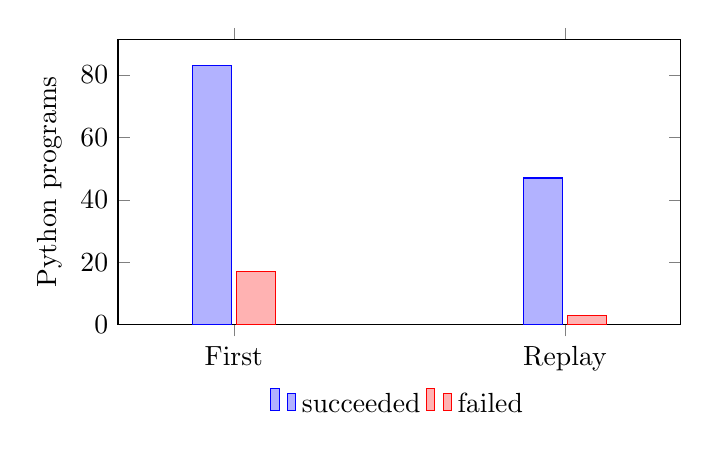
\begin{tikzpicture}
\begin{axis}[
  ybar, bar width=14pt, width=0.72\textwidth, height=5.2cm,
  symbolic x coords={First,Replay}, xtick=data,
  ymin=0, ylabel={Python programs}, enlarge x limits=0.35,
  legend style={at={(0.5,-0.2)},anchor=north,legend columns=2,draw=none},
]
\addplot coordinates {(First,83) (Replay,47)};
\addplot coordinates {(First,17) (Replay,3)};
\legend{succeeded, failed}
\end{axis}
\end{tikzpicture}
\caption{Program outcomes. The replay wrote half as many programs and failed
five times fewer.}
\end{figure}

The drop in programs matters as much as the drop in failures. The model no
longer spends calls discovering the surface. In the first corpus, 31 programs
were tagged as probes: calls to \code{print(a.tools)}, \code{dir()},
\code{inspect.signature}, or reads of the SDK source. The replay has zero. The
prompt now lists exactly the enabled methods, and \code{agent.help()} answers a
signature question without a probe program.

\section{Arms}

\begin{table}[h]
\centering
\footnotesize
\setlength{\tabcolsep}{3.5pt}
\begin{tabular}{@{}lrrrrrrr@{}}
\toprule
& \multicolumn{3}{c}{First corpus} & \multicolumn{3}{c}{Replay} & \\
\cmidrule(lr){2-4}\cmidrule(lr){5-7}
Arm & Time & Programs & Err & Time & Programs & Err & Child calls \\
\midrule
0 & 15.0 & 0/0 & 0 & 40.4 & 0/0 & 0 & 0 \\
A & 157.9 & 20/22 & 2 & 45.1 & 6/6 & 0 & 21 \\
B & 30.1 & 5/6 & 1 & 36.6 & 6/6 & 0 & 7 \\
C & 25.9 & 5/5 & 0 & 47.5 & 8/8 & 0 & 9 \\
D & 53.0 & 11/13 & 2 & 26.5 & 6/6 & 0 & 7 \\
U & 80.5 & 9/11 & 2 & 276.1 & 4/6 & 2 & 73 \\
\bottomrule
\end{tabular}
\caption{Arms. Programs are successes over attempts; errors are failed
programs. Times are seconds.}
\end{table}

\paragraph{A, B, C, D.}
Every sandboxed Python arm finished with zero failed programs. A, B, and D also
became faster and wrote fewer programs: A went from 22 programs to 6, B stayed
at 6 but removed its failure, and D went from 13 to 6. C wrote more programs
(8 against 5) and took longer (47.5 against 25.9), but wrote the same single
deliverable and had no failures.
The reduction is consistent with removing surface discovery, not with doing
less work: each arm still produced \code{index.html}, and the file was read back
inside a program.

\paragraph{Arm 0.}
The native arm took 40.4 seconds against 15.0. It used the native browser tool
17 times, which the first arm did not. It is a native-tool run, not a Python
run; the difference is model choice, not adapter behavior.

\paragraph{Arm U.}
Arm U is the cost centre. It took 276.1 seconds against 80.5 and made 68
\code{browser.call} actions in four successful programs, plus two failed ones.
The final report claims, and the transcript supports, add, complete, delete,
clear-completed, reload persistence, and a clean \code{page.audit()}. The first
U run did not exercise the browser this heavily. The two failures are API
ergonomics, not capability failures, and are analyzed in Section~\ref{sec:fail}.

\section{Scenarios}

\begin{table}[h]
\centering
\footnotesize
\setlength{\tabcolsep}{3pt}
\begin{tabular}{@{}lrrrrrrr@{}}
\toprule
& \multicolumn{3}{c}{First corpus} & \multicolumn{3}{c}{Replay} & \\
\cmidrule(lr){2-4}\cmidrule(lr){5-7}
Scenario & Time & Programs & Err & Time & Programs & Err & Child \\
\midrule
browser\_bwrap & 207.7 & 4/7 & 3 & 11.1 & 2/2 & 0 & 12 \\
browser\_none & 62.7 & 5/9 & 4 & 10.8 & 3/3 & 0 & 9 \\
browser\_text\_bwrap & 6.4 & 1/1 & 0 & 6.3 & 1/1 & 0 & 3 \\
jobs\_bwrap & 4.8 & 1/1 & 0 & 6.9 & 1/1 & 0 & 2 \\
jobs\_none & 9.2 & 2/3 & 1 & 4.2 & 1/1 & 0 & 2 \\
detached\_bwrap & 19.6 & 3/3 & 0 & 16.7 & 2/3 & 1 & 1 \\
detached\_none & 23.5 & 7/8 & 1 & 12.6 & 1/1 & 0 & 1 \\
detached\_none2 & 24.4 & 3/3 & 0 & 55.2 & 2/2 & 0 & 1 \\
combo\_bwrap & 14.0 & 1/1 & 0 & 9.4 & 1/1 & 0 & 3 \\
combo\_none & 16.3 & 4/5 & 1 & 8.2 & 1/1 & 0 & 3 \\
attachments\_bwrap & 9.1 & 1/1 & 0 & 10.5 & 1/1 & 0 & 3 \\
attachments\_none & 9.3 & 1/1 & 0 & 9.8 & 1/1 & 0 & 3 \\
\bottomrule
\end{tabular}
\caption{Capability scenarios. Child is the number of tool calls made inside
Python programs.}
\end{table}

\paragraph{Browser.}
This is the largest change. The old \code{browser\_bwrap} run took 207.7 seconds,
wrote seven programs, failed three, and hit a 30-second \code{wait} timeout and a
schema error. The replay took 11.1 seconds, wrote two programs, failed none, and
returned the title, snapshot, screenshot path, and MIME type. The old
\code{browser\_none} run took 62.7 seconds and failed four programs; the replay
took 10.8 seconds and failed none. The model used the new helpers naturally:
\code{page.title()}, \code{page.screenshot(save=...)}, and the dict-style
\code{shot["mime"]} access that the old run guessed and lost.

\paragraph{Jobs and detached tasks.}
All five job and combo scenarios succeeded without a failure. \code{detached\_}
\code{none2} took 55.2 seconds, against 24.4, because the program returned the
job and then waited for the host's completion notification before the session
ended. That is the scenario's intended behavior, not a stall.

\paragraph{Detached bwrap.}
The only scenario failure was a probe program:
\code{from agent import agents, agent} raised
\code{ImportError: cannot import name 'agent' from 'agent'}. The next program
imported correctly, launched the task, and recovered. The intended work
succeeded.

\paragraph{Attachments.}
Both sandboxes returned the image and the fetched image with MIME types, with
one program each, as before. Times are within a second of the first corpus.

\section{Failure analysis}
\label{sec:fail}

Three programs failed in the replay, against seventeen before.

\begin{table}[h]
\centering
\small
\begin{tabular}{@{}llr@{}}
\toprule
Run & Failure & Count \\
\midrule
U & \code{page.is\_("disabled", ...)}: unknown subcommand & 1 \\
U & \code{page.find\_all(...)[0].check()}: Node has no actions & 1 \\
detached\_bwrap & \code{from agent import agent}: not exported & 1 \\
\bottomrule
\end{tabular}
\caption{Every failed program in the replay.}
\end{table}

The first two are API-shape mismatches, not missing capabilities:

\begin{lstlisting}[style=python]
# The model expected the inverse of `enabled`.
page.is_("disabled", "#add-btn")

# It expected find_all to return actionable elements, as find_one does.
boxes = page.find_all(role="checkbox")
boxes[0].check()
\end{lstlisting}

\code{Page.is\_} accepts only \code{visible}, \code{enabled}, and
\code{checked}. \code{find\_all} returns \code{Node} records; only
\code{find\_one} returns an \code{Element}. Both are defensible designs, and
both invite the guess the model made. Recommended fixes are in
Section~\ref{sec:next}.

The third is a plain import mistake. \code{agent} is injected into a program's
namespace by the loader, but it is not an exported name of the package, so
\code{from agent import agents, agent} fails. One line in
\code{agent/\_\_init\_\_.py} would make the explicit form work.

\begin{table}[h]
\centering
\small
\begin{tabular}{@{}lrr@{}}
\toprule
Error kind & First corpus & Replay \\
\midrule
attribute & 5 & 1 \\
shape misuse & 3 & 0 \\
import & 2 & 0\textsuperscript{*} \\
timeout & 2 & 0 \\
other & 5 & 2 \\
\midrule
total & 17 & 3 \\
\bottomrule
\end{tabular}
\caption{Failed programs by kind. *The \code{cannot import name} message is
classified as other by the shared classifier.}
\end{table}

Shape misuse, timeouts, and missing-module errors disappeared. The old
\code{GlobResult is not iterable}, \code{Text has no total\_lines}, and
\code{Screenshot is not subscriptable} classes of failure are gone; the replay
used \code{shot["mime"]} and \code{find\_one} without incident.

\section{Raw capability audit}
\label{sec:audit}

\begin{table}[h]
\centering
\small
\begin{tabular}{@{}lrr@{}}
\toprule
Counter & First corpus & Replay \\
\midrule
raw open & 0 & 6 \\
raw exec & 0 & 0 \\
raw net & 0 & 0 \\
\bottomrule
\end{tabular}
\end{table}

The six raw opens are all \code{Screenshot.save} writing a PNG:
one in \code{browser\_bwrap}, three in \code{browser\_none}, and two in arm U.
The audit hook records Python's \code{open(..., "wb")} regardless of intent, so
the new helper moves this counter from zero. None is a bypass: the write target
is \code{/tmp} or the workspace, and no process or socket was opened. Future
reports should report \code{rawOpen - screenshotSaves} rather than compare the
raw total directly.

The bwrap arms ran on the real sandbox. The image had lost \code{bubblewrap},
and package metadata was empty, so the harness now installs the Ubuntu 26.04
\code{bubblewrap} and \code{libcap2} debs directly. A smoke run and all four
sandboxed arms and six bwrap scenarios then ran with the sandbox active.

\section{What changed between corpora}

The replay is not only a rerun; it evaluates the ergonomics work described in
\code{analysis/fix-plan.md} and \code{analysis/browser-plan.md}.

\begin{table}[h]
\centering
\small
\begin{tabular}{@{}p{0.34\textwidth}p{0.56\textwidth}@{}}
\toprule
Change & Effect visible in this corpus \\
\midrule
Prompt lists exactly the enabled methods and \code{AgentError} & probe programs fall from 31 to 0; programs halve \\
Loader wraps scripts without \code{Run} and puts modules in scope & several scripts run as written; two would have failed before \\
Dict-style results and field suggestions & \code{shot["mime"]} and \code{.get}; no shape failures \\
Printed output and program-line traces & failures and print output reach the model in one result \\
Error kinds mapped from native messages & no \code{tool\_failed} catch-alls in the replay \\
\code{find\_one} element handles and \code{find\_all} & used for every form interaction; one mismatch remains \\
Typed console, errors, network, tabs, audit & U ran a real QA pass and quoted a clean audit \\
\code{Screenshot.save} and \code{evaluate} decoding & screenshots land in the workspace; no JSON wrapper guesses \\
\code{tab\_select} fix and \code{fs.write} hint & not exercised as failures in this matrix \\
Scratch browser & disabled; not part of this comparison \\
\bottomrule
\end{tabular}
\caption{The independent variable.}
\end{table}

Two changes did not show up as expected. \code{find\_all} still returns nodes,
and the model expected elements. \code{Page.is\_} still lacks the inverse
spellings that read naturally. Both are narrow, and both are cheap to fix.

\section{Threats to validity}

\begin{itemize}[leftmargin=1.3em]
\item \textbf{One run per cell.} The old and new numbers are single samples.
A 45-second arm A and a 158-second arm A could both be normal for the same
configuration. The failure counts are more robust than the times, but even they
have no confidence interval.
\item \textbf{Different work in arm U.} The replay's U run made 68 browser calls
and tested persistence and deletion. The old U run made far fewer. The 276
seconds mostly measure the test pass the model chose, not adapter overhead.
\item \textbf{Prompts are identical, models are not deterministic.} The replay
used the same prompt bytes, but sampling and provider behavior can change.
\item \textbf{Arm 0 is a native-tool run.} Its time changed because the model
used the native browser 17 times. It is not evidence about the Python adapter.
\item \textbf{No visual grading.} The harness checks files, sessions, and audit
counters. It does not score the rendered UI. Arm U's final text claims a
screenshot check; that claim is not independently graded here.
\item \textbf{Export and bwrap changes.} The harness fixes make the replay
possible but also mean the environment is not byte-identical to the first
corpus.
\end{itemize}

\section{Recommended next fixes}
\label{sec:next}

\begin{enumerate}[leftmargin=1.5em]
\small
\item \textbf{Alias the inverse state checks.} Map \code{disabled} to
\code{not enabled} and \code{hidden} to \code{not visible} in
\code{Page.is\_}. This removes one replay failure and one obvious guess.
\item \textbf{Return elements from \code{find\_all}.} Keep \code{nodes()} for
raw records. Then \code{find\_all(role="checkbox")} returns handles, and
\code{[0].check()} works. This removes the second replay failure.
\item \textbf{Export \code{agent} from the package.} Make
\code{from agent import agent} resolve to the package module, or reject it with
a hint. This removes the third failure.
\item \textbf{Account for intentional raw opens.} Report screenshot saves
separately from other \code{raw\_open} events, so the sandbox metric stays
comparable across helper versions.
\item \textbf{Repeat the matrix twice.} One sample per cell cannot separate
prompt effects from run-to-run variance. A second replay, ideally with the same
key and model settings, would make the headline numbers a distribution.
\end{enumerate}

\section{Conclusion}

The current build removed the friction that dominated the first corpus. Half as
many programs were needed, five times fewer failed, the browser scenarios went
from minutes to seconds, and no program hit a shape, timeout, or missing-module
error. The sandbox contract held: no raw executions, no raw sockets, and the only
raw opens were the new screenshot helper writing files it was asked to write.

The remaining failures are small API mismatches, not missing tools. They point to
three one-line fixes and one measurement change. The larger caveat is
statistical: this is a replay of one matrix, not a repeated experiment.

\appendix
\section{Run IDs}
\label{app:runs}

\begin{table}[h]
\centering
\footnotesize
\begin{tabular}{@{}ll@{}}
\toprule
Kind & Replay run IDs \\
\midrule
Arm 0 & \code{0-20261119T175247} \\
Arm A & \code{A-20261119T180934} \\
Arm B & \code{B-20261119T175726} \\
Arm C & \code{C-20261119T175817} \\
Arm D & \code{D-20261119T175942} \\
Arm U & \code{U-20261119T181029} \\
\code{browser\_bwrap} & \code{browser\_bwrap-20261119T180136} \\
\code{browser\_none} & \code{browser\_none-20261119T180157} \\
\code{browser\_text\_bwrap} & \code{browser\_text\_bwrap-20261119T180218} \\
\code{jobs\_bwrap} & \code{jobs\_bwrap-20261119T180252} \\
\code{jobs\_none} & \code{jobs\_none-20261119T180311} \\
\code{detached\_bwrap} & \code{detached\_bwrap-20261119T180354} \\
\code{detached\_none} & \code{detached\_none-20261119T180421} \\
\code{detached\_none2} & \code{detached\_none2-20261119T180452} \\
\code{combo\_bwrap} & \code{combo\_bwrap-20261119T180557} \\
\code{combo\_none} & \code{combo\_none-20261119T180625} \\
\code{attachments\_bwrap} & \code{attachments\_bwrap-20261119T180649} \\
\code{attachments\_none} & \code{attachments\_none-20261119T180751} \\
\bottomrule
\end{tabular}
\caption{Every run used in the comparison. The two superseded arm attempts are
listed in \code{analysis/harness-2026-11-19-replay/README.md}.}
\end{table}

\section{Reproducing}

\begin{verbatim}
OPENCODE_API_KEY=... ./harness/replay-report-2026-11-19.sh all
python3 analysis/aggregate_replay.py
pdflatex report.tex && pdflatex report.tex
\end{verbatim}

The replay script writes one run per arm and scenario under
\code{harness/runs/}. The aggregator reads those run directories and the first
corpus, and writes \code{runs.json}, \code{runs.csv}, and \code{summary.json}
beside this report. The comparison is defined by the run lists in
\code{analysis/aggregate\_replay.py}, so a future replay can be added without
editing the prose tables by hand.

\end{document}
